\documentclass[a4paper,landscape,titlepage,17pt]{extarticle}
\usepackage{color,amsmath,graphicx}
\usepackage[citestyle=numeric,backend=bibtex]{biblatex}
\usepackage[labelfont=bf]{caption}
\usepackage[affil-it]{authblk}
\usepackage{fullpage}
\usepackage{pdflscape}
\linespread{1}
\pagenumbering{gobble}
\bibliography{library}

\title{\Huge Increased concentration of proteins with growth rate can result from passive resource redistribution}
\author{\Large Uri Barenholz, Leeat Keren, Ron Milo}
\affil{The Weizmann Institute of Science, Rehovot, Israel}
\date{}

\begin{document}
\maketitle
\section*{\LARGE Abstract}
In many microorganisms, the proteome composition changes dramatically as a function of the growth environment.
Furthermore, many of these changes seem to be coordinated with the growth rate rather than the specific environment.
However, although cellular growth rates, gene expression levels and gene regulation have been at the center of biological research for decades, their quantitative interdependence is not yet fully understood.

We analyzed the relationship between growth rate and proteome composition for the model microorganism \emph{E.coli} as reflected in two proteomics data sets spanning various growth conditions.
We found that the cellular concentration of a large fraction of the proteins measured coordinately increases with the growth rate.
This fraction includes proteins spanning different functional groups and proteins that are involved in different cellular processes.
Notably, Ribosomal proteins are only a small fraction of this group of proteins.

We present a simple model that demonstrates how such a widely coordinated increase in the concentration of many proteins can be the result of passive redistribution of resources, due to active regulation of a few proteins.
Our model provides a potential explanation for why and how such changes relate to the growth rate under different environmental conditions.
The model thus suggests that, although the concentrations of many proteins change with the growth rate, such changes could be part of a global effect, not requiring specific cellular control mechanisms.
\clearpage        

\begin{figure}[h]
\centering
\includegraphics[scale=1.7]{GrowthRateCorrelation.pdf}
\caption{\linespread{0.5}\selectfont{}
  We analyzed two data sets in which \emph{E.coli} was grown at different growth rates and carbon sources, and its proteome composition was assessed by mass spectrometry (\parencite{Valgepea2013}, left panel, and unpublished data from M. Heinemann's lab, right panel).
The Pearson correlation between the concentration of every protein and the growth rate was calculated for each of these data sets.
We find that a significant fraction of the proteome, spanning distinct functional groups, has a high correlation with the growth rate.
}
\label{fig:growthcorr}
\end{figure}

\clearpage        
\section*{\LARGE Results}
\subsection*{Proteins that are positively correlated with growth rate share a similar, significant response}
We examined how large is the response of the proteins that have a significant positive correlation with the growth rate\footnote{High correlation proteins were defined as those with a Pearson correlation in the range $(0.4,0.8)$ and $(0.8,1)$ for the H and V data sets, respectively.} across the conditions measured (referred to as high correlation proteins).
To this end, we summed up the concentrations of all of the high correlation proteins across the conditions measured and compared their total concentration to the growth rate (Figure \ref{fig:globalgrcorr}).
Both data sets presented a significant response ($\approx 2$ fold change in total concentration across $\approx 5$ fold change of the growth rate) with most of the variability of the total concentration being explained by the growth rate ($R^2$ of $0.75$ in H and $0.99$ in V). 

To examine how similar is the behavior with growth rate for different proteins, we calculated the slope of a linear regression line with the growth rate for that protein (Figure \ref{fig:globalfit}).
The analysis reveals that most proteins respond in a similar manner across the different growth conditions.

\subsection*{Ribosomal proteins share the same response to growth rate as other proteins}
We examined how the response of high correlation proteins relates to the well-studied response of the ribosomal proteins.
We therefore performed the same analysis of slopes, restricting it to ribosomal proteins alone (Figure \ref{fig:globalfit}).
The analysis shows that, on average, high correlation proteins scale in the same way as ribosomal proteins do.
\clearpage        

\begin{figure}[h]
\centering
\includegraphics[scale=1.7]{GlobalClusterGRFit.pdf}
\caption{\linespread{0.5}\selectfont{}
The sum of the concentrations (as fractions out of the proteome) of high correlation proteins in each of the data sets, with linear regression lines, is shown.
High correlation proteins form a large fraction out of the proteome at higher growth rates ($>40\%$ for H and $>50\%$ for V).
}

\label{fig:globalgrcorr}
\end{figure}
\clearpage        
\begin{figure}[h]
\centering
\includegraphics[scale=1.9]{AllProtsVSRibosomalNormalizedSlopes.pdf}
\caption{\linespread{0.5}\selectfont{}
    A histogram of the normalized slopes of the trend lines for every high correlation protein (blue), and for every ribosomal protein (green) is shown for the two data sets analyzed.
    Left panel - data from \parencite{Valgepea2013}, right panel - data from the Heinemann lab.
    High correlation proteins all share a relatively similar response, meaning they maintain their relative ratios.
    Ribosomal proteins respond in a similar manner to the rest of the high correlation proteins .
}
\label{fig:globalfit}
\end{figure}
\clearpage        

\begin{figure}[h]
\centering
\includegraphics[scale=1.9]{HeinmannChemostatGr.pdf}
\caption{\linespread{0.5}\selectfont{}
  Restricting the analysis of the Heinemann data set to chemostat conditions yields similar results to those obtained for the Valgepea data set.
}
\label{fig:growthcorrchemo}
\end{figure}
\clearpage        

\section*{Summary of findings}
\begin{itemize}
\item The concentration of a large fraction of the proteome increases with growth rate (Figures \ref{fig:growthcorr}, \ref{fig:globalgrcorr}).
\item This behavior is shared by functionally distinct groups of genes and quantitatively resembles the previously described increase of ribosomal proteins with growth rate (Figures \ref{fig:growthcorr}, \ref{fig:globalfit}).
\item A similar change with growth rate implies that these proteins maintain proportionality across different conditions.
\end{itemize}

\clearpage        
\subsection*{Theoretical model}
In an attempt to explain how such a wide-span positive response occurs, we have constructed a minimalistic model that is able to reproduce these results as the outcome of redistribution of resources of the bio-synthesis machinery.
Briefly, the model assumes that favorable growth conditions allow the cell to down-regulate some proteins that are needed in harsher conditions, thus reducing the amount of proteins that need to be produced for the cell to proliferate (Figure \ref{fig:model}).
As a consequence, the fraction of each of the rest of the proteins out of the proteome increases, without invoking specific regulation.
The growth rate therefore increases as well, due to the fact that the ratio of bio-synthetic machinery to the rest of the proteome increases.

\clearpage
\begin{landscape}
\begin{figure}[h]
\centering
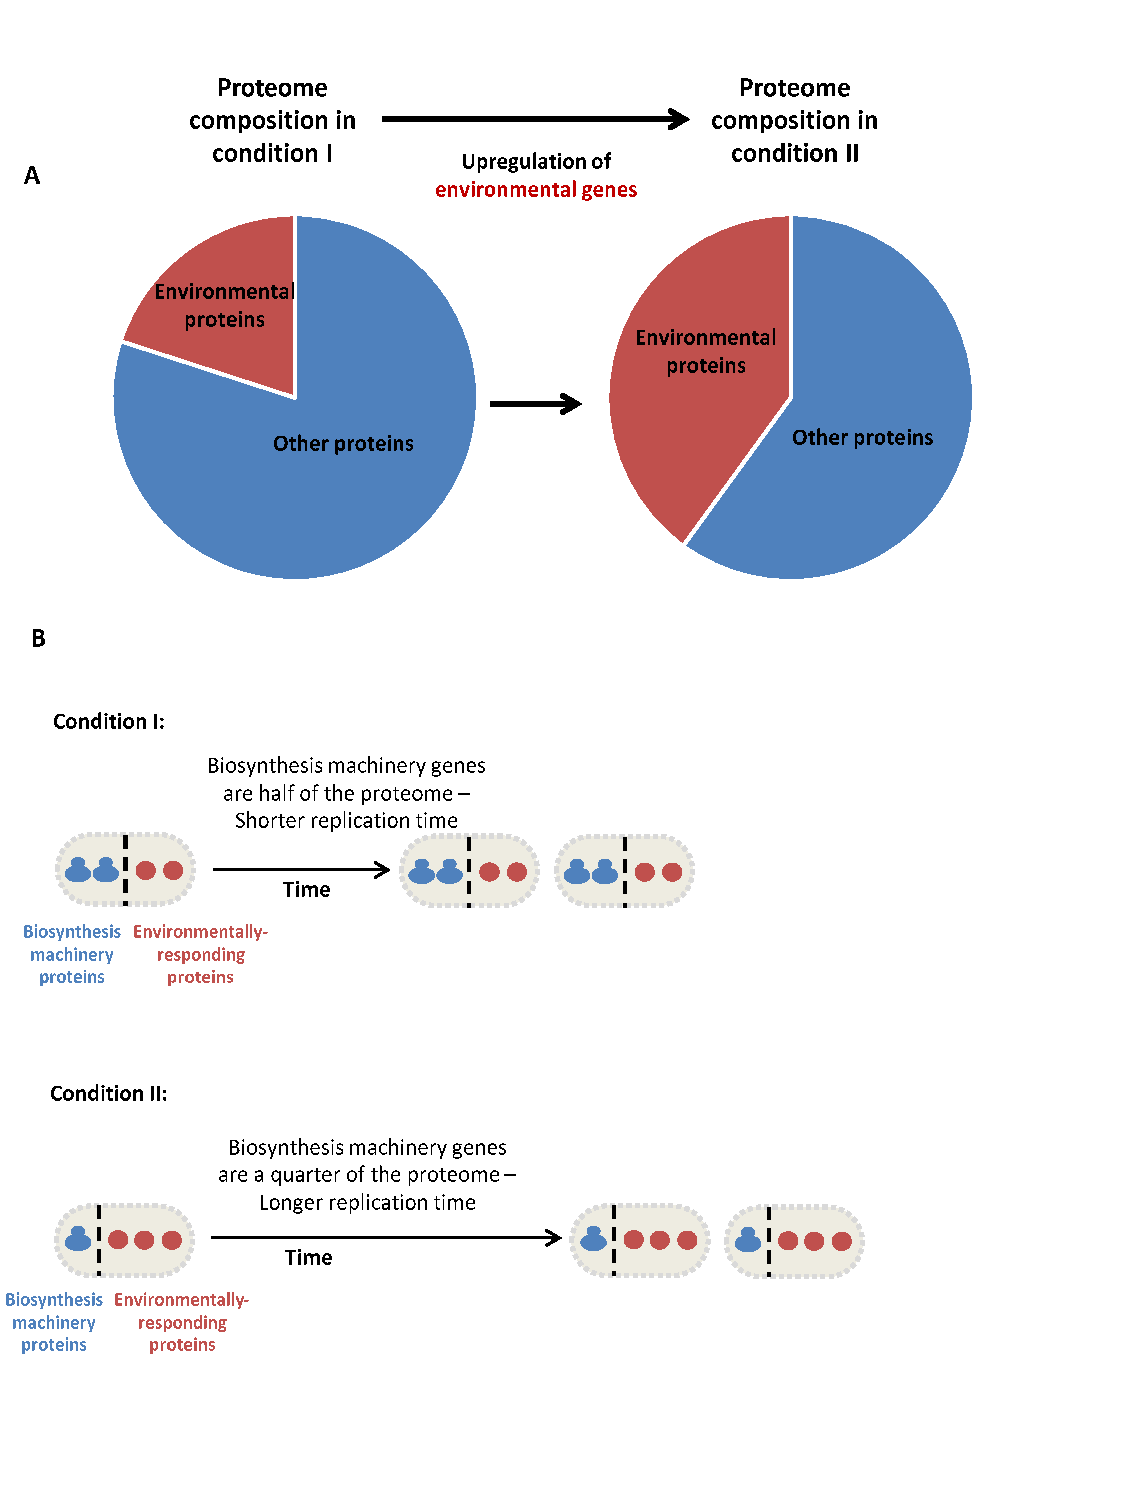
\includegraphics[scale=0.9]{Figures7-trieste.pdf}
\caption{\linespread{0.5}\selectfont{}
  A minimalistic model predicts up regulation of environmental genes reduces the concentration of other proteins (Panel A).
As a result, the ratio of bio-synthesis machinery genes to the rest of the proteome decreases, resulting in slower growth (Panel B).
}
\label{fig:model}
\end{figure}
\end{landscape}
\clearpage        


\printbibliography
\end{document}